\documentclass[12pt, a4paper]{article}
\usepackage{graphicx}
\graphicspath{{pictures/}}
\DeclareGraphicsExtensions{.pdf,.png,.jpg}
\usepackage[utf8]{inputenc}
\usepackage[english,russian]{babel}
\usepackage{amssymb}
\usepackage{amsmath}

\begin{document}
	\begin{titlepage}
		\begin{center}
			\textbf{МИНИСТЕРСТВО ОБРАЗОВАНИЯ РЕСПУБЛИКИ БЕЛАРУСЬ}
		\end{center}
		\begin{center}
			\textbf{БЕЛОРУССКИЙ ГОСУДАРСТВЕННЫЙ УНИВЕРСИТЕТ}
		\end{center}
		\begin{center}
			\textbf{Фaкультет приклaдной мaтемaтики и информaтики}
		\end{center}
		\begin{center}
			Кaфедрa теории вероятностей и мaтемaтической стaтистики
		\end{center}
		\vfill
		\begin{center}
			\large{\bf{Исследование однолинейной системы массового обслуживания с самогенерацией энергии}}
		\end{center}
		\begin{center}
			Курсовой проект
		\end{center}
		
		\vfill
		
		\begin{tabular}{p{80mm}p{90mm}}
			&
			Джига Александра Олеговича\newline
			
			студента 3 курса 7 группы\newline
			
			специальность "прикладная математика"\newline
			
			\textbf{Руководитель}\newline
			
			\textit{Дудин Александр Николаевич}\newline
			
			доктор физико-мaтемaтических нaук, \newline профессор
			\vskip 1em
			
		\end{tabular}
		\vfill
		\vfill
		\begin{center}Минск 2017\end{center}
	\end{titlepage}
\setcounter{page}{2}
\begin{center}
	\section*{Реферат}
	\begin{flushleft}
		$\qquad$Ключевые слова: СИСТЕМА МАССОВОГО ОБСЛУЖИВАНИЯ,
		СИСТЕМА MAP|G|1, ПЕРЕХОДНЫЕ ВЕРОЯТНОСТИ, КРИТЕРИЙ
		ЭРГОДИЧНОСТИ, СТАЦИОНАРНОЕ РАСПРЕДЕНИЯ ВЕРОЯТНОСТЕЙ.\\
		Объектом исследования является система массового обслуживания типа
		$MAP|G|1$ с генерацией энергии. Цель работы – изучить систему, описать модель
		и исследовать ее поведение в различных случаях. Найдены переходные
		вероятности системы. Построена матрица переходных вероятностей. Найдено
		условие эргодичности.
	\end{flushleft}
	\begin{flushleft}
		$\qquad$Ключавыя словы: СIСТЭМА МАСАВАГА АБСЛУГОЎВАННЯ,
		СIСТЭМА MAP | G | 1, ПЕРАХОДНЫЯ IМАВЕРНАСЦI, КРЫТЭРЫЙ
		ЭРГАДЗIЧНАСЦI, СТАЦЫЯНАРНАЕ РАЗМЕРКАВАННЕ IМАВЕРНАСЦЕЎ.\\
		Аб’ектам даследавання з’яўляецца сiстэма масавага абслугоўвання тыпу
		$MAP|G|1$ з генерацыяй энергii. Мэта работы - вывучыць сiстэму, апiсаць мадэль
		i даследаваць яе паводзiны ў розных выпадках. Знойдзеныя пераходныя
		iмавернасцi сiстэмы. Пабудавана матрыца пераходных iмавернасцеў.
		Знойдзена ўмова эргадзічнасці.
	\end{flushleft}
	\begin{flushleft}
		$\qquad$ Key words: QUEUEING SYSTEM, MAP | G | 1 SYSTEM, TRANSITION
		PROBABILITIES, ERGODICITY CRITERION, STATIONARY DISTRIBUTION
		OF PROBABILITIES.\\
		The object of the study is a queuing system of the $MAP|G|1$ type with the
		generation of energy. The aim of the work is to study the system, describe the
		model and investigate its behavior in various cases. The transition probabilities
		of the system are found. A matrix of transition probabilities is constructed. The
		ergodicity condition is found.
		parameters.

	\end{flushleft}
\end{center}
\newpage
\tableofcontents

\newpage
	\large
	\textbf{ВВЕДЕНИЕ}\\
	Математические модели систем массового обслуживания (СМО) широко применяются для исследования и оптимизации процессов в различных физических, экономических, производственных, административных, медицинских, военных и других системах. Объектом исследования в теории СМО являются ситуации, когда имеется некоторый ограниченный ресурс и множество запросов на удовлетворения потребности в этом ресурсе. Примерами могут служить кассы в магазинах, аэропортах, вокзалах и т.д.; терминалы в транспортных системах; банкоматы, инфокиоски и точки оплаты с использованием пластиковых карт; таблицы и индексы реляционных баз данных; ресурсы медицинских, экстренных и аварийных служб; средства радиолокации и противовоздушной обороны; авторизационные серверы в банках, контактные, справочные и информационные центры и т.д. Ограниченность ресурса и случайный характер потока запросов приводят к отказу или задержке в удовлетворении запросов. Стремление уменьшить вероятность этих отказов и длительность задержек и явилось побуждающим мотивом развития теории СМО. С точки зрения используемого математического аппарата, теория СМО может быть классифицирована как прикладная ветвь теории вероятностей, а более точно, теории случайных процессов. Классическая теория СМО основана на использовании известных результатов из теории цепей Маркова с непрерывным временем (и, в частности, теории процессов гибели и размножения) и дискретным временем, теории марковских, полумарковских, линейчатых и близких к ним процессов. Все эти процессы являются одномерными или двумерными (где вторая компонента является непрерывной, носит вспомогательных характер и предназначена для получения марковского процесса).
	
	\section{МАТЕМАТИЧЕСКАЯ МОДЕЛЬ СИСТЕМЫ MAP|G|1 С ГЕНЕРАЦИЕЙ ЭНЕРГИИ}
	\subsection{Математическая модель}
	Поступление единиц энергии подчинено пуассоновскому
	процессу с параметром $\gamma$. Запросы поступают $MAP$ - потоком под управлением
	неприводимой ЦМ с параметром $\nu_{t},\\ t\geq 0$, с непрерывным временем. Время пребывания цепи $\nu_{t}$ в
	некотором состоянии $\nu$ имеет показательное распределение с параметром
	$\lambda_{\nu}$. После того, как время пребывания процесса в этом состоянии
	истекло, с вероятностью $p_{l}(\nu, \nu')$ процесс $\nu_{t}$ переходит (перескакивает) в
	некоторое состояние $\nu'$ и генерируется группа из $l$ запросов, $l =0, 1$. При
	этом $p_{0}(\nu, \nu)$= = 0. Для $MAP$-потока невозможно определить считающую функцию как в стационарном пуассоновском(как безусловную вероятность), поскольку число запросов, поступивших за интервал времени длиной $t$ зависит от состояния управляющего
	процесса $\nu_{t}$, $t\geq $0, в момент начала этого интервала. Но можно вычислить
	вероятности $P_{\nu, \nu'}(l , t)$
	(за время $t$ поступит $l$ запросов и $\nu_{t} = \nu'$ при условии $\nu_{0} = \nu$).

	Вероятность поступления 0 запросов за время $t$ имеет вид $P(0, t) = e^{D_{0}t}$.  Здесь $D_{k}$ – квадратные матрицы порядка $W + 1$, элементы которых определяются следующим образом:

	$$(D_0)_{\nu,\nu'}=\left\{
	\begin{array}{rcl}-\lambda_\nu, &\nu=\nu',\\\lambda_\nu p_0(\nu,\nu'),
	&\nu\neq\nu',
	\end{array}\right.$$
	$$(D_k)_{\nu,\nu'}=\lambda_\nu p_k(\nu,\nu'), k\geq 1,
	$$
	$D(z) = D_{0} + D_{1}z$.\\
	 Запросы поступают 
	в прибор в порядке FIFO. Время обслуживания прибора имеет функцию
	распределения $B(t)$.\\
	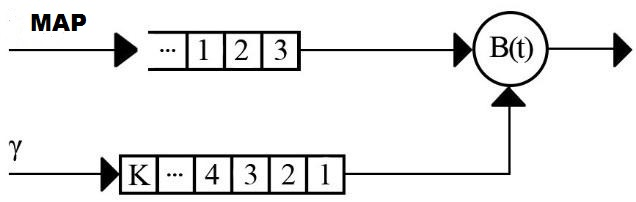
\includegraphics{img139}\\
	Для обслуживания одного запроса необходима одна единица энергия. Единица энергии
	берется сразу после того, как запрос поступит на обслуживание.  Если же буфер
	для хранения энергии пуст, то система переходит в режим ожидания
	до тех пор, пока не поступит единица энергии. Если буфер энергии заполнен,
	то поступающие единицы энергии теряются.\newpage
	\subsection {Необходимые обозначения}

Вероятность поступление в буфер $k$ единиц энергии за время $t$:

$\phi_{k}(t) = \frac{(\gamma t)^{k} }{k!} e^{-\gamma t}, k \geq 0$.

Вероятность поступление в буфер не менее $k$ единиц энергии за время $t$:

$\ \hat\phi_{k}(t) = \sum\limits_{i=k}^{\infty} \phi_{i}(t), k \geq 0$.

Вероятность поступления $k$ единиц энергии за время обслуживания одной заявки:

$\ \phi_{k} =   \int\limits_{0}^{\infty}\phi_{k}(t)dB(t),\ k \geq 0$.

Сумма вероятностей поступления не менее $k$ единиц энергии за время обслуживания одной заявки: 

$\ \hat\phi_{k} = \sum\limits_{i=k}^{\infty} \phi_{i}, k \geq 0$.

Матрица вероятностей поступления $i$ заявок и  $k$ единиц энергии за время обслуживания одной заявки:

$\ \Phi(i, k) =  \int\limits_{0}^{\infty} P(i,t)\phi_{k}(t)dB(t), i \geq 0, k \geq 0$.

 Матрица вероятностей поступления $i$ заявок и не менее $k$ единиц энергии за время обслуживания одной заявки:
 
$\ \hat\Phi(i, k) = \int\limits_{0}^{\infty}  P(i, t) \hat\phi_{k}(t)dB(t), i \geq 0, k \geq 0$.

Матрица вероятностей того, что за время отсутствия единиц энергии в буфере поступит $n$ запросов:

$\ N(n) = \int\limits_{0}^{\infty} P(n, t)\gamma e^{-\gamma t}dt$.

Матрица вероятностей того, что за время отсутствия запросов поступит $n$ единиц энергии:

$\ M(n) = \int\limits_{0}^{\infty} e^{D_{0}t}\phi_{n}(t)D_{1}dt = 
	\int\limits_{0}^{\infty} e^{D_{0}t}\frac{(\gamma t)^{n} }{n!} e^{-\gamma I t}D_{1}dt = \gamma(-D_{0} + + \gamma I)^{-(n+1)}D_{1}
$.

Матрица вероятностей того, что за время отсутствия запросов в буфере поступит не менее $m$ единиц энергии: 

$\ \hat M(m) = \sum\limits_{n=m}^{\infty} M(n)$.\\

\subsection{Переходные вероятности}
Данный процесс является немарковским. Для его исследования применим метод вложенных ЦМ. Будем
рассматривать поведение СМО $(i_{t}, k_{t})$, в моменты $t_{n}, \; n\geq1$ окончания  обслуживания запросов, а именно, рассмотрим процесс
$\epsilon_{n} = \left\{i_{n}, k_{n}, \nu_{n}\right\}$ - трехмерный процесс, где $i_{n} = i_{t_{n+0}},\; k_{n} = k_{t_{n-0}},\; \nu_{n} = \nu_{t_{n}}.$
Данный процесс является трехмерной цепью Маркова. Введем матрицу $$P\left\{(i,k) \rightarrow (j, k')\right\},$$ ($\nu\nu'$)-й элемент которой есть вероятность одношагового перехода: $$P\left\{ (i ,k, \nu) \rightarrow (j, k', \nu') )\right\} =$$  $$=P\left\{i_{n+1} = j, k_{n+1} = k', \nu_{n+1} = \nu' |i_{n} = i, k_{n} = k, \nu_{n} = \nu \right\}$$
Нахождение переходных вероятностей в частных случаях проводится путем анализа поведения цепи Маркова между моментами $t_{n}$ и $t_{n+1}$ и использования формулы полной вероятности.$\\$ 
\textbf{Лемма}\\
Матрицы $P\left\{(i,k) \rightarrow (j, k')\right\}$ вычисляются следующим образом:

$P\left\{(0, 0) \rightarrow (j, k' ) \right\}=$\\
$=M(0)\sum\limits_{n = 0}^{j}N(n)\Phi(j-n, k') + N(0)\sum\limits_{m = 0}^{k'}M(m)\Phi(j, k' - m),\\ j\geq 0,\; k' \in [0, K-1]$.

$P\left\{(0, 0) \rightarrow (j, K) \right\}=$\\
$=M(0)\sum\limits_{n = 0}^{j}N(n)\hat\Phi(j-n, K) + N(0)(\sum\limits_{m = 0}^{K}M(m)\hat\Phi(j, K - m) + \hat M(K)\hat \Phi(j, 1)),  j\geq 0.$

$P\left\{(0, k) \rightarrow (j, k') \right\}=$\\
$ =\sum\limits_{m = 0}^{k'-k+1}M(m)\Phi(j,k' - k + 1 - m), j\geq 0,\; k' \geq k-1.$

$P\left\{(0, k) \rightarrow (j, K)\right\}=$\\
$= \sum\limits_{m = 0}^{K-k+1}M(m) \hat \Phi(j, K - k + 1 - m) + \hat M(K - k + 1)\hat \Phi(j, 1),\\ j\geq 0,\; k \leq K$.

$P\left\{(i, 0) \rightarrow (j, k')  \right\}=$\\
$= \sum\limits_{n = 0}^{j - i + 1}N(n)\Phi(j - i + 1 - n, k'),\; i, j\geq 0, i \geq j-1, k' \in [0, K-1] $.

$P\left\{(i, 0) \rightarrow (j, K) \right\}=$\\
$ =\sum\limits_{n = 0}^{j - i + 1}N(n)\hat \Phi(j - i + 1 - n, K),\; i \geq 0,0 \leq i-1 \leq j $.

$P\left\{(i, k) \rightarrow (j, k') \right\}=$\\
$ =\Phi(j - i + 1, k' - k),\; i, j\geq 0,\;j\geq i-1,\; k' \geq k + 1$.

$P\left\{(i, k) \rightarrow (j, K)\right\}=$\\
$= \hat \Phi(j - i + 1, K - k),\; i, j\geq 0,\;j\geq i-1,\; 0 \leq k \leq K $.

\section{Построение матрицы переходных вероятностей}

\subsection{Матрица вероятностей переходов}
Матрица $P$ вероятностей одношаговых переходов рассматриваемого
процесса имеет следующую форму $P = (P_{i,j})i,j \geq 0$. Можно показать, что
матрицы $P_{i,j}$ не зависят от $i$ и $j$, а зависят только от $j - i$. Тогда
обозначим матрицы $(P_{i,j})i=0,\; j \geq 0$  как $ V_{j}$, элементами которых будут переходные
вероятности $P\left\{(0, k) \rightarrow (j, k') \right\}$, где $ k, k' \in [0, K]$. Заметим, что для $i \geq 1$ выполняется следующее:\\
$(P_{i, j-i+1},\: j\geq 0) = (P_{ij}),\: j \geq 0 .\\$
Матрицы $P_{i,i + j - 1}\: i\neq 0,\: j \geq 0,$ в свою очередь, обозначим как $Y_{j},$ элементами которых
будут переходные вероятности $P\left\{(1, k) \rightarrow (j, k') \right\}$ , где $ k, k' \in [O,K]$. Матрица
вероятностей одношаговых переходов $P$ имеет следующую структуру: \\
$P=\begin{bmatrix}
V_{0} & V_{1} & V_{2} & V_{3} & V{_4} & \ldots\\
Y_{0} & Y_{1} & Y_{2} & Y_{3} & Y{_4} & \ldots\\
0 & Y_{0} & Y_{1} & Y_{2} & Y_{3} & \ldots\\
0 & 0 & Y_{0} & Y_{1} & Y_{2} & \ldots\\
\vdots & \vdots & \vdots & \vdots & \vdots & \ddots\\
\end{bmatrix}$\\
Матрицу, имеющие такую структуру, называют блочной верхне-Хессенберговой. Величина скачка вниз компоненты $i_{n}$ за один шаг не превосходит
единицы.

\subsection{Вид матриц $V_{j}$}
Матрицы $V_{j}$ имеют следующий вид: \\
$\begin{bmatrix}
v^{j}_{00} & v^{j}_{01} & v^{j}_{02} & v^{j}_{03} & \ldots & v^{j}_{0K}\\
v^{j}_{10} & v^{j}_{11}& v^{j}_{12} & v^{j}_{13}& \ldots& v^{j}_{1K}\\
0& v^{j}_{21}& v^{j}_{22}& v^{j}_{23}& \ldots & v^{j}_{2K}\\
0& 0& v^{j}_{32}& v^{j}_{33}& \ldots &v^{j}_{3K}\\
\vdots & \vdots & \vdots & \vdots & \ddots & \vdots\\
0 & 0 & 0 & 0 & \ldots  & v^{j}_{KK}\\
\end{bmatrix}$\\\\
Где $v^{j}_{kk'}$ находятся следующим образом:\\
$a.\;v^{j}_{0k'} = P\left\{(0, 0) \rightarrow (j, k') \right\} = M(0)\sum\limits_{n = 0}^{j}N(n)\Phi(j - n, k') +\\ + N(0)\sum\limits_{m = 0}^{k'}M(m)\Phi(j, k' - m),\\
b.\;v^{j}_{kk'} = P\left\{(0, k) \rightarrow (j, k') \right\} = \sum\limits_{m = 0}^{k'-k+1}M(m)\Phi(j, k' - k + 1 - m),\\
c.\;v^{j}_{kK} = P\left\{(0, k) \rightarrow (j, K) \right\} = \sum\limits_{m = 0}^{K-k+1}M(m) \hat \Phi(j, K - k + 1- \\- m) + \hat M(K - k + 1)\hat \Phi(j, 1).\\
$
Проанализировав вид $v^{j}_{kk'}$ сделаем вывод, что, начиная со второй строки,
элементы не зависят от $k$ и $k'$, а зависят только $k' - k$.
\subsection{Вид матриц $Y_{j}$}
Матрицы $Y_{j}$ имеют следующий вид: \\
$\begin{bmatrix}
y^{j}_{00} & y^{j}_{01}& y^{j}_{02}& y^{j}_{03}& \ldots & y^{j}_{0K}\\
y^{j}_{10} & y^{j}_{11}& y^{j}_{12}& y^{j}_{13}& \ldots & y^{j}_{1K}\\
0 & y^{j}_{21}& y^{j}_{22}& y^{j}_{23}& \ldots & y^{j}_{2K}\\
0& 0& y^{j}_{32}& y^{j}_{33}& \ldots & y^{j}_{3K}\\
\vdots & \vdots & \vdots & \vdots & \ddots & \vdots\\
0 & 0 & 0 & 0 & \ldots & y^{j}_{KK}\\
\end{bmatrix}$\\ \\
Где $y^{j}_{kk'}$ находятся следующим образом:\\
$
a.\;y^{j}_{0k'} = P\left\{(1, 0) \rightarrow (j, k') \right\} = \sum\limits_{n = 0}^{j - 2}N(n)\Phi(j - 2 - n, k'),\\
b.\;y^{j}_{kk'} = P\left\{(1, k) \rightarrow (j, k') \right\} = \Phi(j, k' - k + 1) ,\\
c.\;y^{j}_{kK} = P\left\{(1, k) \rightarrow (j, K) \right\} = \hat \Phi(j, K - k + 1) .\\
$
Проанализировав вид $y^{j}_{kk'}$ сделаем вывод, что, начиная со второй строки,
элементы не зависят от $k$ и $k'$, а зависят только $k' - k$.
\section{СТАЦИОНАРНОЕ РАСПРЕДЕЛЕНИЕ ВЕРОЯТНОСТЕЙ}
\subsection{КРИТЕРИЙ ЭРГОДИЧНОСТИ СИСТЕМЫ}
Условие эргодичности можно трактовать следующим образом - 
условие, при котором система способна уменьшать число заявок в системе,
когда она перегружена, т.е. среднее число заявок, поступающих за время
обслуживания одной заявки, должно быть меньше единицы.\\
Введем матричные ПФ $V(z) = \sum\limits_{i = 0}^{\infty}V_{i}z^{i}$, $\;Y(z) = \sum\limits_{i = 0}^{\infty}Y_{i}z^{i}$, где $V_{j} = P_{0,i+j-1} и Y_{j} = P_{i,i+j-1}$\\
$Y(z) = \sum\limits_{j = 0}^{\infty}Y_{j}z^{j} =  \int\limits_{0}^{\infty}\sum\limits_{j = 0}^{\infty}z^{j}P(j, t)\frac{(\gamma t)^{k} }{k!}e^{-\lambda t}dB(t)$ =\\
$=\int\limits_{0}^{\infty}e^{D(z)t}\phi_{k}(t)dB(t)$, где $D(z) = D_{0} + D_{1}z$\\
\textbf{Теорема}\\
Пусть ЦМ $\epsilon_{n} = \left\{i_{n}, k_{n}, \nu_{n}\right\}$, с матрицей переходных вероятностей P является неприводимой и апериодической, матрицы $Y(1)$ и $V(1)$ являются стохастическими и неприводимыми и выполняются неравенства $V'(1) < \infty$ и $Y'(1) < \infty$. Для того, чтобы ЦМ $\epsilon_{n},\; n\geq 1$, была эргодичной, необходимо и достаточно, чтобы выполнялось неравенство:\\
$$[det(zl - Y(z))]'_{z=1} > 0     \eqno(1)\\$$
\textbf{Следствие}\\
Неравенство (1) эквивалентно следующему неравенству:\\
$\vec{y}\sum\limits_{k = 1}^{\infty}kY_{k}(1)e\;<\;1$,\\
где вектор $\vec{y}$ удовлетворяет системе уравнений:\\
$
\begin{cases}
\vec{y}\sum\limits_{k = 0}^{\infty}Y_{k}(1) = \vec{y}\\
\vec{y}e = 1.
\end{cases}\\
$
Пусть вектор $y$ имеет вид \\
$$y = \theta\otimes u\eqno(2)$$
где ${\theta}$ - вектор стационарного распределения процесса $MAP$ $\nu_t,\,t\geq0,$ и $u= (u_{1}, u_{2}, . . . , u_{K})$.
Найдем вектор u. Компоненты вектора u
удовлетворяют следующей системе алгебраических уравнений:\\
$
\begin{cases}
u_{k+1} = u_{0}\phi_{k} + \sum\limits_{s=1}^{k+1}u_{s}\phi_{k + 1 - s}, k = \overline{0, K-1},\\
u_{K} = u_{0}\hat\phi{k} + \sum\limits_{s=1}^{K}u_{s}\phi_{K + 1 - s}.
\end{cases}\\
$
Решим эту систему, представив $u_{k}$ следующим образом:\\
$
\begin{cases}
	u_{k} = u_{0}\psi_{k}\\
	u_{K} = (\sum\limits_{k=0}^{K}\psi_{k})^{-1},
\end{cases}\\
$
Где $\psi_{k}$:\\
$\psi_{k+1}\; =\;\psi_{k} - \phi_{k} - \sum\limits_{s=1}^{k}\psi_{s}\phi_{k + 1 - s}, k = \overline{1, K-1}, $\\
После подстановки $u$ и $y$ получаем условие эргодичности:\\
$\lambda b_{1} + u_{0}  \frac{\lambda}{\gamma}\; <\; 1$,\\
где $b_{1}$ это время обслуживания одной заявки.\\
Условие существования стационарного режима в системе совпадает с условием
эргодичности вложенной цепи Маркова. 
\begin{flushleft}\subsection{Матрично-аналитический метод для нахождения стационарного распределения вероятностей цепи Маркова (метод М. Ньютса)}\end{flushleft}

Краеугольным понятием в подходе М. Ньютса является понятие фундаментального периода. Фундаментальный период — это интервал времени с момента, когда значение счетной компоненты равно $i$, до первого момента, когда значение этой компоненты станет равным $i - 1$, $i \geq 1$. Из определения ЦМ типа $MAP|G|1$ следует, что длина фундаментального периода не зависит от значения $i$. 

Обозначим $G(z)$ матричную ПФ, $(k, k')$-й элемент которой есть ПФ числа переходов, осуществленных ЦМ за фундаментальный период, который закончился, когда значение конечной компоненты есть $k'$ при условии, что в момент начала фундаментального периода значение конечной компоненты равнялось $k$; $k, k' = \overline{0, K}$ . Используя факты из теории марковских процессов восстановления, можно показать, что матрица $G(z)$ удовлетворяет уравнению

\begin{equation}
\label{eq5}
G(z) = z \sum\limits_{j = 0}^{\infty} Y_j G^j(z).
\end{equation}

Обозначим через $G^{(i)}$ матрицу вероятностей переходов компоненты $k_n$ за время первого достижения первой компонентой $i_n$ значения $i$, начиная с $i + 1$.

Используя формулу полной вероятности, нетрудно убедиться, что матрицы $G^{(i)}, i \geq 0$, удовлетворяют уравнениям

\begin{equation}
\label{eq6}
G^{(i)} = P_{i + 1, i} + \sum\limits_{l = i + 1}^{\infty} P_{i + 1, l} G^{(l - 1)} G^{(l - 2)} \ldots G^{(i)}, i \geq 0.
\end{equation}

Учитывая квазитеплицевость рассматриваемой ЦМ, можно заключить, что матрицы $G^{(i)}, i \geq 0$, не зависят от $i$. Пусть все они равны некоторой матрице $G$. Тогда из (\ref{eq6}) можно заключить, что матрица $G$, удовлетворяет уравнению 

\begin{equation}
\label{eq7}
G = \sum\limits_{j = 0}^{\infty} Y_j G^j.
\end{equation}

Отметим, что уравнение (\ref{eq5}) автоматически следует из уравнения (\ref{eq7}), поскольку из определения матриц $G$ и $G(z)$ следует, что $G(1) = G$.

Обозначим через $\pi_i, i \geq 0$, векторы стационарных вероятностей исходной ЦМ $\xi_n, n \geq 1$.

\begin{equation}
\label{eq8}
\pi_j = \sum\limits_{i = 0}^{j} \pi_i \overline{P}_{i, j}, i \geq 0, 
\end{equation}

где матрицы $\overline{P}_{i, j}$ задаются уравнениями

\begin{equation}
\label{eq9}
\overline{P}_{i, j} = P_{i, j} + \sum\limits_{l = j + 1}^{\infty} P_{i, l} G^{l - j}, j \geq i. 
\end{equation}

Из (\ref{eq8}) следует, что векторы $\pi_i, i \geq 0$, стационарных вероятностей можно представить в виде

\begin{equation}
\label{eq10}
\pi_i = \pi_0 \Phi_i, i \geq 0, 
\end{equation}

где матрицы $\Phi_i, i \geq 0$ удовлетворяют рекуррентным соотношениям

\begin{equation}
\label{eq11}
\Phi_0 = I, \Phi_l = \left(\overline{P}_{0, l} + \sum\limits_{i = 1}^{l - 1} \Phi_i \overline{P}_{i, l}\right) \left(I - \overline{P}_{l, l}\right)^{-1}, l \geq 1.
\end{equation}

Соотношения (\ref{eq10}) определяют векторы $\pi_i, i \geq 0$, стационарных вероятностей с точностью до неизвестного пока вектора $\pi_0$. Этот вектор можно вычислить через аппарат векторных ПФ или по формуле (\ref{eq12}). Однако, предположим еще одну процедуру для подсчета вектора $\pi_0$.

Из уравнений (\ref{eq8}) при $j = 0$ получаем:

\begin{equation}
\label{eq12}
\pi_0(I - \overline{P}_{0, 0}) = 0. 
\end{equation}

Домножением соотношения (\ref{eq9}) справа на вектор $e$ несложно убедиться, что матрица $\overline{P}_{0, 0}$ - стохастическая. По построению эта матрица является неприводимой, поэтому ранг системы (\ref{eq12}) на единицу меньше размерности вектора $\pi_0$. Значит, система (\ref{eq12}) определяет вектор $\pi_0$ с точностью до некоторой константы. Следовательно, если нам удастся получить еще одно, неоднородное, уравнение для компонент вектора $\pi_0$, то полученнная система будет иметь единственное решение. Такое уравнение легко получается из (\ref{eq10}) и условия нормировки и имеет вид: 

\begin{equation}
\label{eq13}
\pi_0 \sum\limits_{i = 0}^{\infty} \Phi_i e = 1. 
\end{equation}

Подводя итог, сформулируем следующий алгоритм нахождения векторов $\pi_i, i \geq 0$, стационарных вероятностей:

\vspace{10pt}
\begin{enumerate}
	\item Находим матрицу $G$ как решение нелинейного матричного уравнения (\ref{eq7}).
	\item Вычисляем матрицы $\overline{P}_{i, l}$ по формулам (\ref{eq9}).
	\item Вычисляем матрицы $\Phi_l$ по рекуррентным формулам (\ref{eq11}).
	\item Находим вектор $\pi_0$ как единственное решение системы (\ref{eq12}), (\ref{eq13}).
	\item Ищем необходимое число векторов $\pi_i$ по формулам (\ref{eq10}).
\end{enumerate}
\pagebreak

\begin{flushleft}
	\section{АНАЛИЗ ХАРАКТЕРИСТИК ПРОИЗВОДИТЕЛЬНОСТИ СИСТЕМЫ}
\end{flushleft}
\setcounter{equation}{0}
\setcounter{figure}{0}
\setcounter{table}{0}

\subsection{Среднее количество запросов в системе}


Обозначим среднее количество запросов в системе как $L$. Найдем $L$ по следующей формуле:

$$L = \sum\limits_{i = 0}^{\infty} i \pi_i e.$$

Построим график $L$ для значений $k$ $($от $1$ до $K$ с шагом $1)$ и  $T$ $($от $0.5$ до $1.5$  с шагом $0.5)$.

\begin{figure}[h]
	\center{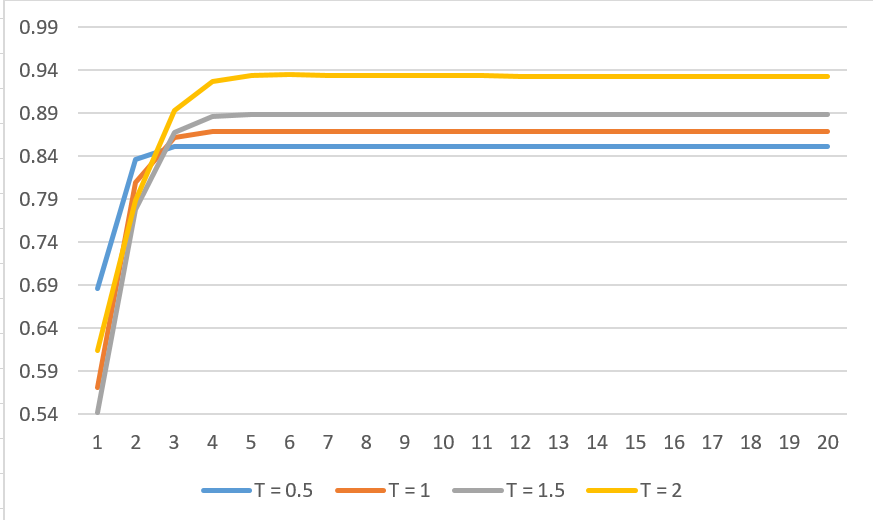
\includegraphics[scale=1.0]{11.png}}
	\caption{Среднее количество запросов в системе}
	\label{ris2}
\end{figure}


Среднее количество запросов в системе увеличивается по мере возрастания времени обслуживания. \pagebreak

\textbf{Входные данные:}

$\lambda: 0.4$

$\gamma: 0.3$

$K: 1, 2, 3, \ldots, 20$

$T: 0.5, 1.0, 1.5$

$Accuracy: 0.001$

\begin{figure}[h]
	\center{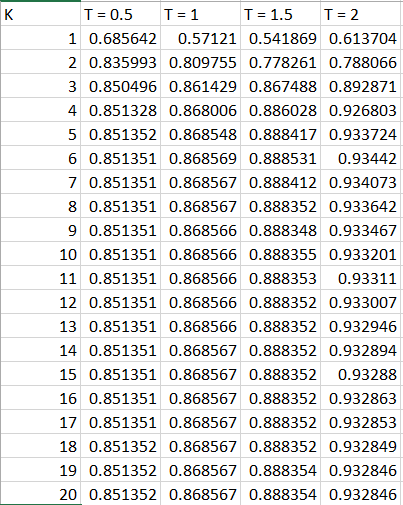
\includegraphics[scale=1.0]{1.png}}
\end{figure}

\begin{flushleft}\subsection{Среднее количество единиц энергии в буфере}\end{flushleft}

Обозначим среднее количество единиц энергии в буфере как $N$. Найдем $N$ по следующей формуле:

$$N =\sum\limits_{i = 0}^{\infty} \sum\limits_{k = 1}^{K} k \pi(i, k)e,$$ где $\pi_i = (\pi(i, 0), \pi(i, 1), \ldots, \pi(i, K)).$

Построим график $N$ для значений $k$ $($от $1$ до $K$ с шагом $1)$ и  $T$ $($от $0.5$ до $1.5$  с шагом $0.5)$.

\begin{figure}[h]
	\center{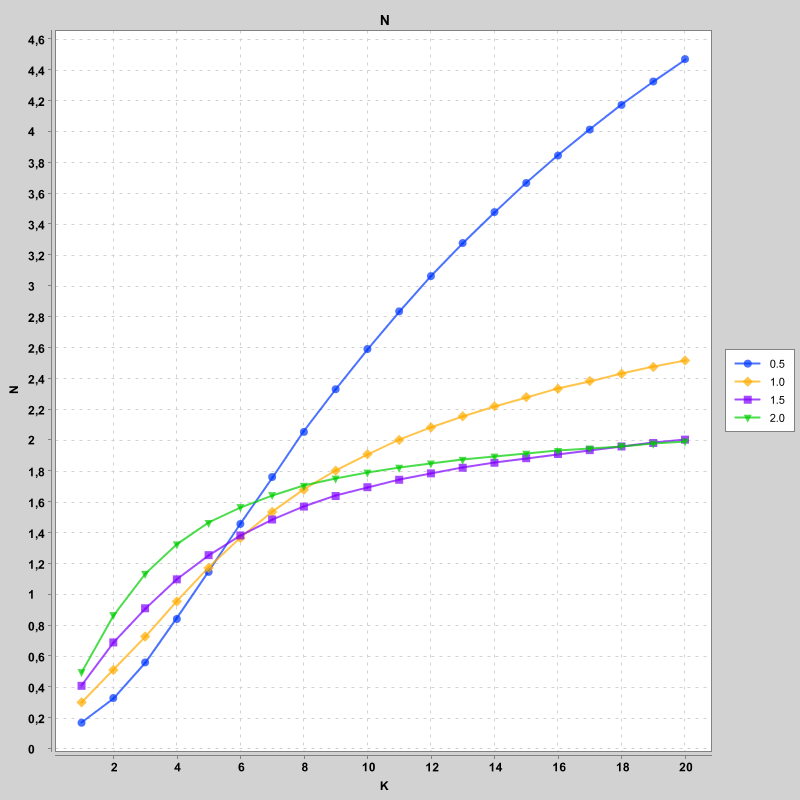
\includegraphics[scale=1]{12.png}}
	\caption{Среднее количество единиц энергии в буфере}
	\label{ris3}
\end{figure}

Среднее количество единиц энергии в буфере увеличивается с возрастанием времени обслуживания в системе. 
\pagebreak

\textbf{Входные данные:}

$\lambda: 0.4$

$\gamma: 0.3$

$K: 1, 2, 3, \ldots, 20$

$T: 0.5, 1.0, 1.5$

$Accuracy: 0.001$

\begin{figure}[h]
	\center{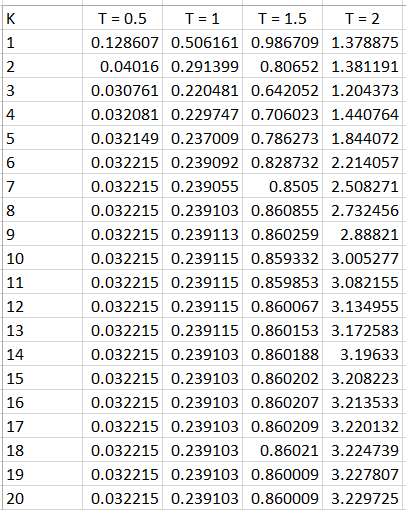
\includegraphics[scale=1]{2.png}}
\end{figure}

\pagebreak

\subsection{Вероятность отсутствия запросов в системе}


Обозначим вероятность того, что заявок в системе нет как $P_0^{custom}$. Найдем $P_0^{custom}$ по следующей формуле:

$$P_0^{custom} = \pi_0 e.$$

Построим график $P_0^{custom}$ для значений $k$ $($от $1$ до $K$ с шагом $1)$ и  $T$ $($от $0.5$ до $1.5$  с шагом $0.5)$.
\begin{figure}[h]
	\center{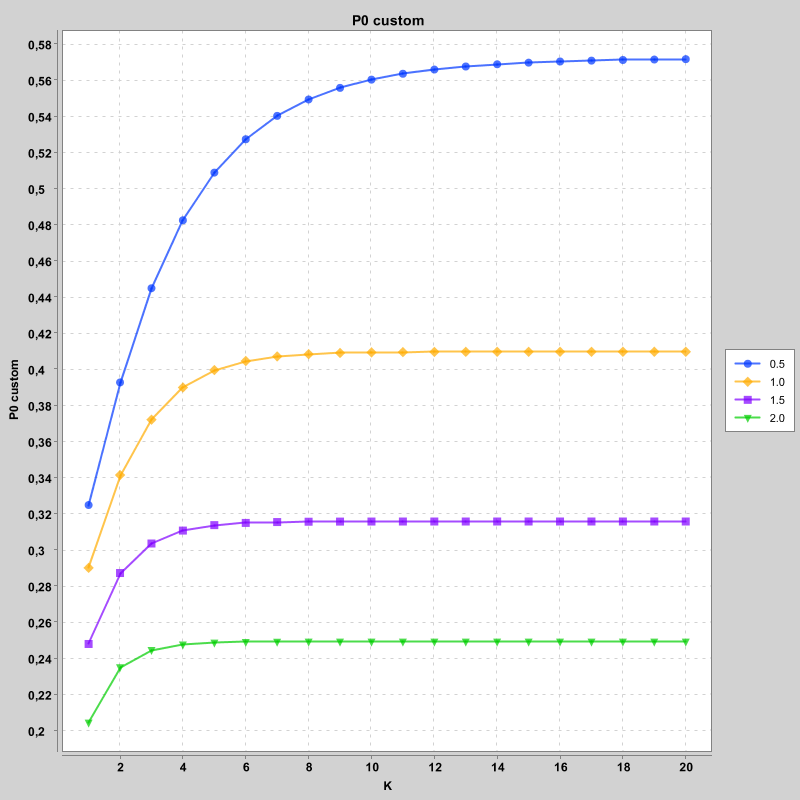
\includegraphics[scale=1]{13.png}}
	\caption{Вероятность отсутствия запросов в системе}
	\label{ris4}
\end{figure}


Вероятность отсутствия запросов в системе увеличивается по мере уменьшения времени обслуживания запросов.

\pagebreak
\textbf{Входные данные:}

$\lambda: 0.4$

$\gamma: 0.3$

$K: 1, 2, 3, \ldots, 20$

$T: 0.5, 1.0, 1.5$

$Accuracy: 0.001$

\begin{figure}[h]
	\center{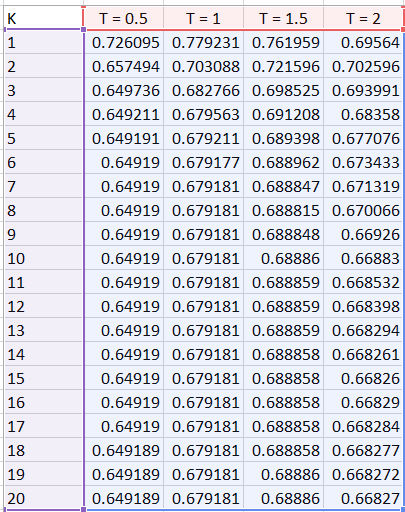
\includegraphics[scale=1]{3.png}}
\end{figure}


	\subsection{Вероятность отсутствия единиц энергии в буфере}


Обозначим вероятность отсутствия единиц энергии в буфере как $P_0^{energy}$. Найдем $P_0^{energy}$ по следующей формуле:

$$P_0^{energy} = \sum\limits_{i = 0}^{\infty} \pi(i, 0)e,$$ где $\pi_i = (\pi(i, 0), \pi(i, 1), \ldots, \pi(i, K))$

Построим график $P_0^{energy}$ для значений $k$ $($от $1$ до $K$ с шагом $1)$ и  $T$ $($от $0.5$ до $1.5$  с шагом $0.5)$.

\begin{figure}[h]
	\center{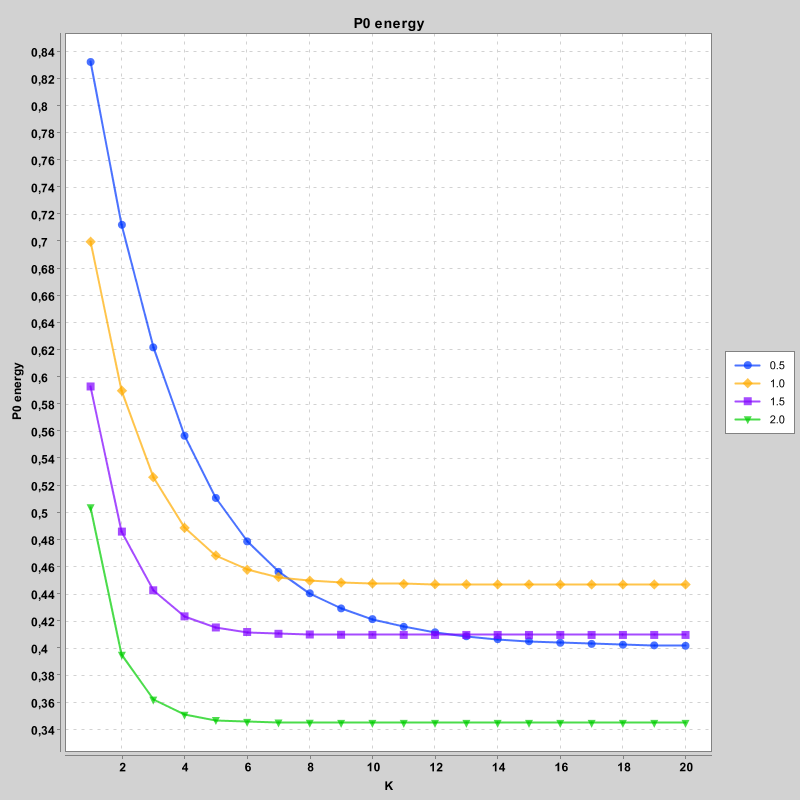
\includegraphics[scale=1]{14.png}}
	\caption{Вероятность отсутствия единиц энергии в буфере}
	\label{ris5}
\end{figure}

Вероятность отсутствия единиц энергии в буфере увеличивается по мере уменьшения времени обслуживания заявок системой. 

\pagebreak
\textbf{Входные данные:}

$\lambda: 0.4$

$\gamma: 0.3$

$K: 1, 2, 3, \ldots, 20$

$T: 0.5, 1.0, 1.5$

$Accuracy: 0.001$

\begin{figure}[h]
	\center{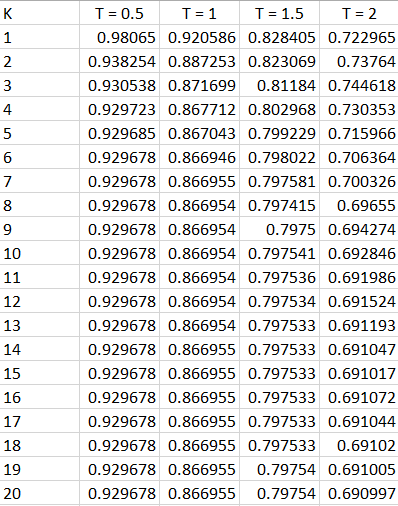
\includegraphics[scale=1]{4.png}}
\end{figure}

\pagebreak
\begin{flushleft}\subsection{Вероятность простоя системы по причине отсутствия единиц энергии в буфере}\end{flushleft}

Обозначим вероятность простоя системы по причине отсутствия единиц энергии в буфере как $P_{idle}$. Найдем $P_{idle}$ по следующей формуле:

$$P_{idle} = \sum\limits_{i = 1}^{\infty} \pi(i, 0)e,$$ где $\pi_i = (\pi(i, 0), \pi(i, 1), \ldots, \pi(i, K)).$

Построим график $P_{idle}$ для значений $k$ $($от $1$ до $K$ с шагом $1)$ и  $T$ $($от $0.5$ до $1.5$  с шагом $0.5)$.
\begin{figure}[h]
	\center{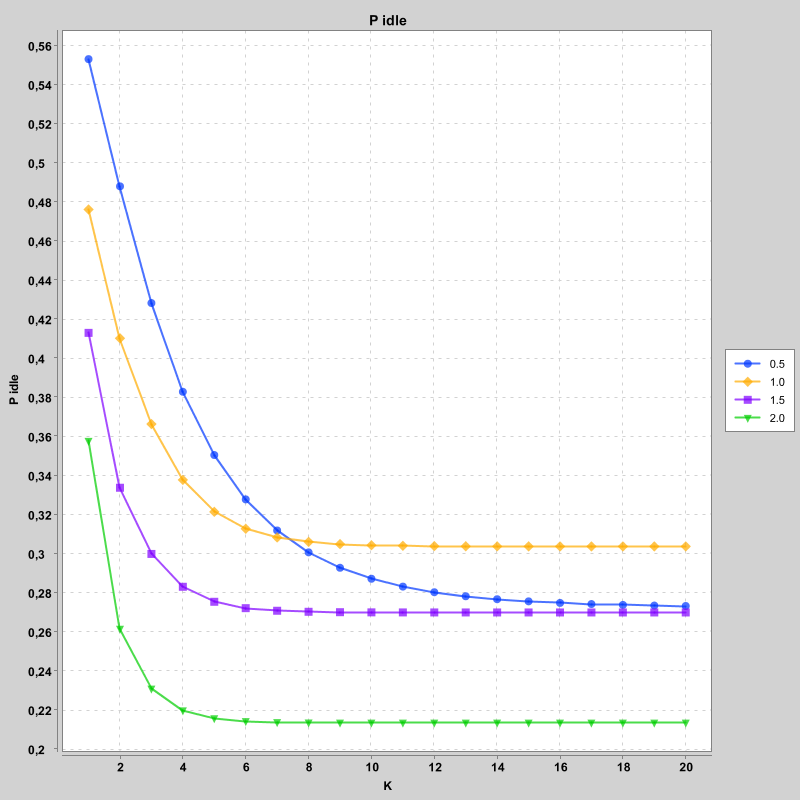
\includegraphics[scale=1]{15.png}}
	\caption{Вероятность простоя системы по причине отсутствия единиц энергии в буфере}
	\label{ris6}
\end{figure}

Вероятность простоя системы по причине отсутствия единиц энергии в буфере возрастает с уменьшением времени обслуживания. Другими словами - единицы энергии потребляются быстрее, что приводит к увеличению шанса простоя системы.

\pagebreak
\textbf{Входные данные:}

$\lambda: 0.4$

$\gamma: 0.3$

$K: 1, 2, 3, \ldots, 20$

$T: 0.5, 1.0, 1.5$

$Accuracy: 0.001$

\begin{figure}[h]
	\center{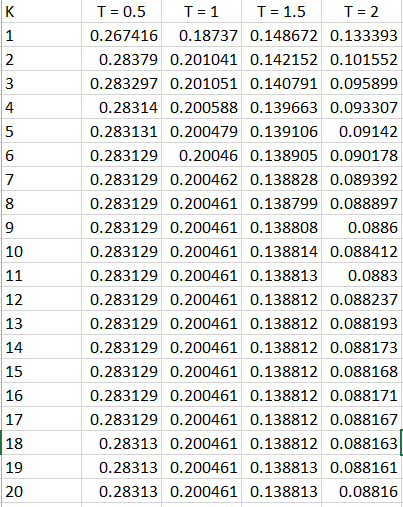
\includegraphics[scale=1]{5.png}}
\end{figure}
\pagebreak
\begin{flushleft}\subsection{Вывод по итогам анализа характеристик производительности}\end{flushleft}

Путем сравнения характеристик производительности и выявления особенностей поведения системы можно повысить ее эфективность, повлияв на определенные параметры. Стоит отметить, что увеличение объема буфера энергии далеко не всегда способствует улучшению значения соответствующей характеристики т.к., начиная с опроеделенного значения $K$, это теряет всякий смысл, изменения достаточно малы и это не окажет существенного влияния на работу системы.

Стоит добавить, что при исследовании системы при значениях $T > 2.0$ условие эргодичности начинает выполняться только для достаточно больших значений $K$.

\pagebreak
\begin{center}
	\section*{ЗАКЛЮЧЕНИЕ}
\end{center}
\addcontentsline{toc}{section}{ЗАКЛЮЧЕНИЕ}

В процессе выполнения курсовой работы:

\begin{flushleft}
	\begin{enumerate}
		\item Исследована система массового обслуживания типа $M|G|1$. Найдены вероятности одношаговых переходов, а так же построена матрица переходных вероятностей. Проверено выполнение условия эргодичности и на основе этого найдено стационарное распределение вероятностей.
		\item Разработана программная реализация предложенного метода нахождения стационарного распределения вероятностей на языке программирования Java.
		\item На основе программной реализации метода нахождения стационарного распределения вероятностей найдены характеристики производительности искомой системы. Произведен их анализ и сделаны выводы. 
	\end{enumerate}
\end{flushleft}
\newpage
\begin{thebibliography}{20}
	\bibitem{KlDud}
	Klimenok, V.I., Dudin A.N.:  Multi-dimensional asymptotically quasi-Toeplitz Markov
	chains and their application in queueing theory.  Queueing Systems, ~54,  245--259 (2006)
	\bibitem{kd}
	Klimenok  V.I.,   Dudin A.N.  Multi-dimensional asymptotically quasi-Toeplitz
	Markov chains and their application in queueing theory // Queueing
	Systems. 2006. V. 54. P. 245-259.
\end{thebibliography}
\pagebreak
\begin{center}\section*{ПРИЛОЖЕНИЕ А}\end{center}
\addcontentsline{toc}{section}{ПРИЛОЖЕНИЕ А}
\begin{enumerate}
	\item \textbf{Класс для создания матриц $Y_i$, $V_i$}
	
	\begin{verbatim}
	package core;
	
	import kurs.BigDecimalMatrix;
	
	import java.math.BigDecimal;
	import java.math.RoundingMode;
	
	import static java.math.BigDecimal.ONE;
	import static java.math.BigDecimal.ZERO;
	
	
	public class GeneratorCreator {
	private BigDecimal gamma;
	private BigDecimal lambda;
	private Integer K;
	private BigDecimal accuracy;
	private BigDecimalMatrix d0;
	private BigDecimalMatrix d1;
	private BigDecimal T;
	private MatrixElementCreator elementCreator;
	
	public GeneratorCreator(
	BigDecimal gamma,
	BigDecimal lambda,
	int K,
	BigDecimalMatrix d0,
	BigDecimalMatrix d1,
	BigDecimal T,
	BigDecimal accuracy
	) {
	boolean validness = gamma.compareTo(ONE) < 0 &&
	gamma.compareTo(ZERO) > 0 &&
	lambda.compareTo(ONE) < 0 &&
	lambda.compareTo(ZERO) > 0 &&
	K > 0 &&
	gamma.compareTo(lambda) > 0;
	
	if(!ErgodicityCondition.check(gamma, lambda, K, T)) {
	throw new IllegalArgumentException("Ergodicity condition does not perform. " + T + " " + K);
	}
	if (!validness) {
	throw new IllegalArgumentException("Input parameters are not valid.");
	}
	
	this.gamma = gamma;
	this.lambda = lambda;
	this.K = K;
	this.accuracy = accuracy;
	this.d0 = d0;
	this.T = T;
	this.d1 = d1;
	this.elementCreator = new MatrixElementCreator();
	}
	
	public BigDecimalMatrix[][] create(int i, int j) {
	BigDecimalMatrix[][] matrix = new BigDecimalMatrix[K + 1][K + 1];
	
	if (i - j > 1) {
	return matrix;
	}
	
	for (int r = 0; r < K + 1; r++) {
	for (int c = 0; c < K + 1; c++) {
	matrix[r][c] =  elementCreator.create(i, r, j, c);
	//System.out.println(matrix[r][c]);
	}
	}
	
	return matrix;
	}
	
	private class MatrixElementCreator {
	
	//Approved
	private BigDecimalMatrix create(int i, int k, int j, int bK) {
	boolean validness = i >= 0 &&
	j >= 0 &&
	k >= 0 &&
	k <= K &&
	bK >= 0 &&
	bK <= K;
	if (!validness) {
	throw new IllegalArgumentException("Indexes out of bounds.");
	}
	
	BigDecimalMatrix element;
	if (k - bK > 1) {
	element = new BigDecimalMatrix(2, 2, 10);
	} else if (k == 0) {
	if (bK == K) {
	element = createLastColumnElement(i, k, j, bK);
	} else {
	element = createFirstRowNotLastColumnElement(i, k, j, bK);
	}
	} else {
	if (bK == K) {
	element = createLastColumnElement(i, k, j, bK);
	} else {
	element = createNotFirstRowNotLastColumnElement(i, k, j, bK);
	}
	}
	//System.out.println(element);
	return element;
	}
	private BigDecimalMatrix createFirstRowNotLastColumnElement(int i, int k, int j, int bK) {
	BigDecimalMatrix result = new BigDecimalMatrix(2, 2, 10);
	for(int n = 0; n <= j - 2; n++) {
	result = result.add(
	funcN(n).multiply(funcPhi(new BigDecimal(j - 2 - n), new BigDecimal(bK)))
	);
	}
	return result;
	}
	
	//Approved
	private BigDecimalMatrix createLastColumnElement(int i, int k, int j, int bK) {
	return funcPhiWithHat(new BigDecimal(j), new BigDecimal(bK - k + 1));
	}
	
	//Approved
	private BigDecimalMatrix createNotFirstRowNotLastColumnElement(int i, int k, int j, int bK) {
	return funcPhi(new BigDecimal(j), new BigDecimal(bK - k + 1));
	}
	}
	
	public BigDecimalMatrix funcMWithHat(int m) {
	int n = m;
	BigDecimalMatrix mWithHat = new BigDecimalMatrix(2, 2, 10);
	BigDecimalMatrix mn = funcM(n);
	while(Math.sqrt(mn.squaredEuclidianNorm().doubleValue()) >= accuracy.doubleValue()) {
	mWithHat = mWithHat.add(mn);
	n++;
	mn = funcM(n);
	}
	return mWithHat;
	}
	
	public BigDecimalMatrix funcM(int n) {
	BigDecimalMatrix minusD0 = d0.multiply(new BigDecimal(-1));
	BigDecimalMatrix gammaI = new BigDecimalMatrix(2, new BigDecimal(1), 10).multiply(gamma);
	BigDecimalMatrix sumInverse = minusD0.add(gammaI).inverse();
	BigDecimalMatrix val = sumInverse;
	for(int i = 0; i < n; i++) {
	val = val.multiply(sumInverse);
	}
	return val.multiply(gamma.pow(n)).multiply(d1);
	}
	
	public BigDecimalMatrix funcK(int n, int j) {
	if (j == 0) {
	return n == 0 ? new BigDecimalMatrix(2, new BigDecimal(1), 10) : new BigDecimalMatrix(2, 2, 10);
	} else {
	if (n == 0) {
	BigDecimalMatrix sum = new BigDecimalMatrix(2, new BigDecimal(1), 10)
	.add(d0.multiply(new BigDecimal(1)
	.divide(tetta(), RoundingMode.HALF_UP)));
	sum = funcK(0, j - 1).multiply(sum);
	return sum;
	} else {
	BigDecimalMatrix sum = new BigDecimalMatrix(2, 2, 10);
	for (int i = 0; i <= n - 1; i++) {
	if( n - i == 1) {
	sum = sum.add(funcK(i, j - 1).multiply(d1));
	}
	sum = sum.add(funcK(n, j - 1)
	.multiply(new BigDecimalMatrix(2, new BigDecimal(1), 10)
	.add(d0.multiply(new BigDecimal(1).divide(tetta(), RoundingMode.HALF_UP)))));
	}
	return sum.multiply(new BigDecimal(1).divide(tetta(), RoundingMode.HALF_UP));
	}
	}
	}
	
	public BigDecimalMatrix funcP(int n, BigDecimal t) {
	BigDecimalMatrix sum = new BigDecimalMatrix(2, 2, 10);
	BigDecimalMatrix val;
	int j = 1;
	do {
	//val = funcK(j, n);
	val = funcK(n, j);
	val = val.multiply(new BigDecimal(Math.exp(tetta().multiply(new BigDecimal(-1)).multiply(t).doubleValue())))
	.multiply((tetta().multiply(t)).pow(j)
	.divide(factor(new BigDecimal(j)), RoundingMode.HALF_UP));
	sum = sum.add(val);
	j++;
	} while (Math.sqrt(val.squaredEuclidianNorm().doubleValue()) >= accuracy.doubleValue());
	return sum;
	}
	
	public BigDecimal funcSmalPhiK(BigDecimal t, int k) {
	return (gamma.multiply(t).pow(k))
	.divide(factor(new BigDecimal(k)), RoundingMode.HALF_UP)
	.multiply(new BigDecimal(Math.exp(gamma.multiply(t).doubleValue())));
	}
	
	public BigDecimal funcSmalPhiKWithHat(BigDecimal t, int k) {
	BigDecimal val = funcSmalPhiK(t, k);
	BigDecimal result = ZERO;
	int i = k;
	while(val.compareTo(accuracy) == 1 ) {
	result = result.add(val);
	i++;
	val = funcSmalPhiK(t, i);
	}
	return result;
	}
	
	public BigDecimalMatrix funcPhi(BigDecimal i, BigDecimal k) {
	return funcP(i.intValue(), T).multiply(funcSmalPhiK(T, k.intValue()));
	}
	
	public BigDecimalMatrix funcPhiWithHat(BigDecimal i, BigDecimal k) {
	return funcP(i.intValue(), T).multiply(funcSmalPhiKWithHat(T, k.intValue()));
	}
	
	public BigDecimalMatrix funcN(int n) {
	return funcP(n, T).multiply(gamma
	.multiply(new BigDecimal(Math.exp(gamma.multiply(new BigDecimal(-1)).multiply(T).doubleValue()))));
	}
	
	private BigDecimal factor(BigDecimal n) {
	if (n.signum() < 0) {
	throw new IllegalArgumentException("Negative value in factorial function.");
	}
	if (n.scale() < 0) {
	throw new IllegalArgumentException("Real value in factorial function.");
	}
	if (n.equals(ZERO)) {
	return ONE;
	}
	return n.multiply(factor(n.subtract(ONE)));
	}
	
	private BigDecimal tetta() {
	BigDecimal tetta = ZERO;
	for (int i = 0; i < d0.getHeight(); i++) {
	tetta = (d0.getElement(i, i).multiply(new BigDecimal(-1)).compareTo(tetta) == 1) ? d0.getElement(i, i).multiply(new BigDecimal(-1)) : tetta;
	}
	return tetta;
	}
	
	public BigDecimal getAccuracy() {
	return new BigDecimal(accuracy.toString());
	}
	public int getK() {
	return K;
	}
	}
	
	\end{verbatim}
	\pagebreak
	\item \textbf{Класс для проверки условия эргодичности}
	
	\begin{verbatim}
	
	package core;
	
	
	import java.math.BigDecimal;
	import java.math.RoundingMode;
	
	import static java.math.BigDecimal.ONE;
	import static java.math.BigDecimal.ZERO;
	import static java.math.BigDecimal.valueOf;
	
	
	public class ErgodicityCondition {
	
	//Approved
	public static boolean check(BigDecimal gamma, BigDecimal lambda, Integer K, BigDecimal T) {
	BigDecimal minuend = lambda.multiply(T);
	BigDecimal subtrahend = getY0(gamma, T, K).multiply(lambda.divide(gamma, RoundingMode.HALF_UP));
	return minuend.subtract(subtrahend).compareTo(ONE) < 0;
	}
	
	private static BigDecimal getY0(BigDecimal gamma, BigDecimal T, Integer K) {
	BigDecimal[] psiVector = getPsiVector(gamma, T, K);
	BigDecimal sum = ZERO;
	for (BigDecimal element : psiVector) {
	sum = sum.add(element);
	}
	return ONE.divide(sum, RoundingMode.HALF_UP);
	}
	
	//Approved
	private static BigDecimal[] getPsiVector(BigDecimal gamma, BigDecimal T, Integer K) {
	BigDecimal[] psiVector = new BigDecimal[K];
	psiVector[0] = ONE;
	
	for (int k = 0; k < K - 1; k++) {
	BigDecimal sum = ZERO;
	for (int s = 1; s <= k; s++) {
	sum = sum.add(psiVector[s].multiply(smallPhi(gamma, T, valueOf(k + 1 - s))));
	}
	psiVector[k + 1] = psiVector[k].subtract(smallPhi(gamma, T,valueOf(k))).subtract(sum);
	}
	return psiVector;
	}
	
	
	//Approved
	private static BigDecimal smallPhi(BigDecimal gamma, BigDecimal T, BigDecimal k) {
	return (gamma.multiply(T).pow(k.intValue()))
	.divide(factor(k), RoundingMode.HALF_UP)
	.multiply(new BigDecimal(Math.exp(gamma.multiply(T).doubleValue()*-1)));
	}
	
	//Approved
	private static BigDecimal factor(BigDecimal n) {
	if(n.signum() < 0) {
	throw new IllegalArgumentException("Negative value in factorial function.");
	}
	if(n.scale() < 0) {
	throw new IllegalArgumentException("Real value in factorial function.");
	}
	if(n.equals(ZERO)) {
	return ONE;
	}
	return n.multiply(factor(n.subtract(ONE)));
	}
	}
	\end{verbatim}
	\pagebreak
	\item \textbf{Класс для нахождения матриц $G$}
	
	\begin{verbatim}
	package core;
	
	/**
	* Created by Lenovo on 12.05.2018.
	*/
	
	import java.math.BigDecimal;
	import kurs.BigDecimalMatrix;
	
	
	public class GMatrixCreator {
	
	private GeneratorCreator creator;
	private BigDecimal accuracy;
	
	public GMatrixCreator(GeneratorCreator creator) {
	this.creator = creator;
	this.accuracy = creator.getAccuracy();
	}
	
	public BigDecimalMatrix create(BigDecimalMatrix g0) {
	int size = g0.getWidth();
	BigDecimalMatrix gPrev, cur, prev;
	BigDecimalMatrix gCur = new BigDecimalMatrix(size, new BigDecimal(1), 10);
	try {
	do {
	int k = 0;
	gPrev = gCur.clone();
	cur = BigDecimalMatrix.zeroMatrix(size);
	do {
	prev = cur.clone();
	cur = cur.add(per(creator.create(1, k)).multiply(powMatrix(gPrev, k)));
	//System.out.println(per(creator.create(1, k)));
	k++;
	} while (cur.subtract(prev).squaredEuclidianNorm().compareTo(accuracy) > 0);
	gCur = cur.clone();
	} while (gCur.subtract(gPrev).squaredEuclidianNorm().compareTo(accuracy) > 0);
	MatrixContainer.setG(gCur.clone());
	} catch (CloneNotSupportedException e) {
	System.out.println(e.getMessage());
	}
	// System.out.println(gCur.getWidth());
	return gCur;
	}
	public static BigDecimalMatrix per(BigDecimalMatrix[][] a) {
	int size = a.length * 2;
	BigDecimalMatrix cur = BigDecimalMatrix.zeroMatrix(size);
	for (int i = 0; i < a.length; i++) {
	for(int j = 0; j < a[i].length; j++) {
	BigDecimalMatrix val = a[i][j];
	//System.out.println(a[i][j]);
	for (int k = 0; k <= 1; k++) {
	for (int r = 0; r <= 1; r++) {
	cur.setElement(k + i*2, r + j*2, val.getElement(k, r));
	}
	}
	}
	}
	//System.out.println(cur);
	return cur;
	}
	//Approved
	private BigDecimalMatrix powMatrix(BigDecimalMatrix a, int b) {
	if (b < 0) {
	throw new IllegalArgumentException("Negative argument in factorial function.");
	}
	if (b == 0) {
	return BigDecimalMatrix.identity(a.getWidth());
	}
	return a.multiply(powMatrix(a, b - 1));
	}
	}
	
	\end{verbatim}
	\pagebreak
	\item \textbf{Класс для нахождения матриц $\Phi_i$}
	
	\begin{verbatim}
	package core;
	
	import java.math.BigDecimal;
	import java.util.ArrayList;
	import java.util.Objects;
	
	import core.MatrixContainer;
	import kurs.BigDecimalMatrix;
	import java.math.BigDecimal;
	import java.util.ArrayList;
	import java.util.Objects;
	
	public class PhiMatrixCreator {
	private ArrayList<BigDecimalMatrix> phiMatrices;
	private PSlashMatrixCreator pSlashCreator;
	private BigDecimal accuracy;
	private Integer K;
	
	//Approved
	public PhiMatrixCreator(PSlashMatrixCreator pSlashCreator, Integer K) {
	phiMatrices = new ArrayList<>();
	this.pSlashCreator = pSlashCreator;
	this.K = K;
	this.accuracy = pSlashCreator.getAccuracy();
	}
	
	//Approved
	public ArrayList<BigDecimalMatrix> getPhiMatrices() {
	initPsiMatrices();
	return phiMatrices;
	}
	
	//Approved
	private void initPsiMatrices() {
	final BigDecimalMatrix I = BigDecimalMatrix.identity(2*K + 2);
	phiMatrices.add(0, I);
	int hash = Objects.hash(0);
	try {
	if (!MatrixContainer.getPhiMatrices().containsKey(hash)) {
	MatrixContainer.getPhiMatrices().put(hash, I.clone());
	}
	int index = 1;
	BigDecimalMatrix leftTerm;
	BigDecimalMatrix rightTerm;
	BigDecimalMatrix result;
	do {
	hash = Objects.hash(index);
	if (MatrixContainer.getPhiMatrices().containsKey(hash)) {
	phiMatrices.add(index, MatrixContainer.getPhiMatrices().get(hash).clone());
	} else {
	//.inverse()
	rightTerm = I.subtract(pSlashCreator.create(index, index)).inverse();
	
	
	int i = 1;
	leftTerm = BigDecimalMatrix.zeroMatrix(K*2 + 2);
	//System.out.println(1);
	while (i < index) {
	leftTerm = leftTerm.add(phiMatrices.get(i).multiply(pSlashCreator.create(i, index)));
	i++;
	}
	leftTerm = leftTerm.add(pSlashCreator.create(0, index));
	result = leftTerm.multiply(rightTerm);
	//System.out.println(result.squaredEuclidianNorm());
	phiMatrices.add(index, result);
	MatrixContainer.getPhiMatrices().put(hash, result.clone());
	}
	index++;
	//System.out.println(Math.sqrt(phiMatrices.get(index - 1).subtract(phiMatrices.get(index - 2)).squaredEuclidianNorm().doubleValue()));
	} while (phiMatrices.get(index - 1).subtract(phiMatrices.get(index - 2)).squaredEuclidianNorm().compareTo(accuracy) > 0);
	} catch (CloneNotSupportedException e) {
	System.out.println(e.getMessage());
	}
	}
	}
	\end{verbatim}
	\pagebreak
	\item \textbf{Класс для нахождения матриц $\overline{P}_{i, j}$}
	
	\begin{verbatim}
	package core;
	
	import kurs.BigDecimalMatrix;
	
	import java.math.BigDecimal;
	import java.util.Objects;
	
	
	public class PSlashMatrixCreator {
	private GeneratorCreator creator;
	private BigDecimalMatrix g;
	private BigDecimal accuracy;
	
	//Approved
	public PSlashMatrixCreator(GeneratorCreator creator, BigDecimalMatrix g) {
	this.g = g;
	this.creator = creator;
	this.accuracy = creator.getAccuracy();
	}
	
	public BigDecimalMatrix create(Integer i, Integer j) {
	if(j < i) {
	throw new IllegalArgumentException("Index i is bigger than index j in PSlashMatrixCreator.");
	}
	
	int l = j + 1;
	int size = g.getWidth();
	//System.out.println(size);
	int hash = i > 1 ? Objects.hash(1, j - i + 1) : Objects.hash(0, j);
	
	BigDecimalMatrix result = BigDecimalMatrix.zeroMatrix(size);
	
	try {
	if(MatrixContainer.getPSlashMatrices().containsKey(hash)) {
	result = MatrixContainer.getPSlashMatrices().get(hash).clone();
	} else {
	BigDecimalMatrix prev;
	BigDecimalMatrix cur = BigDecimalMatrix.zeroMatrix(size);
	do {
	prev = cur.clone();
	cur = cur.add(GMatrixCreator.per(creator.create(i, l)).multiply(powMatrix(g, l - j)));
	l++;
	} while (cur.subtract(prev).squaredEuclidianNorm().compareTo(accuracy) > 0);
	result = GMatrixCreator.per(creator.create(i, j)).add(cur);
	MatrixContainer.getPSlashMatrices().put(hash, result.clone());
	}
	} catch (CloneNotSupportedException e) {
	System.out.println(e.getMessage());
	}
	return result;
	}
	
	//Approved
	public BigDecimal getAccuracy() {
	return accuracy;
	}
	
	
	//Approved
	private BigDecimalMatrix powMatrix(BigDecimalMatrix a, int b) {
	if (b < 0) {
	throw new IllegalArgumentException("Negative argument in factorial function.");
	}
	if (b == 0) {
	return BigDecimalMatrix.identity(a.getWidth());
	}
	return a.multiply(powMatrix(a, b - 1));
	}
	}
	
	
	\end{verbatim}
	\pagebreak
	\item \textbf{Класс для нахождения векторов $\pi_i$}
	
	\begin{verbatim}
	package core;
	
	import java.math.BigDecimal;
	import java.util.ArrayList;
	import java.util.Objects;
	import kurs.BigDecimalMatrix;
	
	public class StationaryDistributionCreator {
	private PSlashMatrixCreator pSlashCreator;
	private ArrayList<BigDecimalMatrix> phiMatrices;
	private Integer K;
	private ArrayList<BigDecimalMatrix> piVectors;
	
	public StationaryDistributionCreator(PSlashMatrixCreator pSlashCreator, ArrayList<BigDecimalMatrix> phiMatrices, Integer K) {
	this.pSlashCreator = pSlashCreator;
	this.phiMatrices = phiMatrices;
	this.K = K;
	this.piVectors = new ArrayList<>(phiMatrices.size());
	}
	
	public ArrayList<BigDecimalMatrix> getPiVectors() {
	//System.out.println(pSlashCreator.create(0, 0).getWidth());
	BigDecimalMatrix A = BigDecimalMatrix.identity(2*K + 2).subtract(pSlashCreator.create(0, 0));
	BigDecimalMatrix IWaved = BigDecimalMatrix.identity(2*K + 2);
	IWaved.setElement(0, 0, BigDecimal.ZERO);
	
	BigDecimalMatrix eWaved = BigDecimalMatrix.eRow(2*K + 2, BigDecimal.ZERO);
	eWaved.setElement(0, 0, BigDecimal.ONE);
	
	BigDecimalMatrix e = BigDecimalMatrix.eCol(2*K + 2, BigDecimal.ONE);
	BigDecimalMatrix sum = BigDecimalMatrix.zeroMatrix(2*K + 2);
	
	for (BigDecimalMatrix phi : phiMatrices) {
	sum = sum.add(phi.multiply(e).multiply(eWaved));
	}
	
	BigDecimalMatrix AWaved = A.multiply(IWaved).add(sum);
	
	BigDecimalMatrix pi0 = eWaved.multiply(AWaved.inverse());
	BigDecimalMatrix a = new BigDecimalMatrix(2, K + 1, 30);
	for(int j = 0; j < pi0.getWidth(); j += 2) {
	a.setElement(0, j/2, pi0.getElement(0, j));
	a.setElement(1, j/2, pi0.getElement(0, j + 1));
	}
	piVectors.add(0, a);
	MatrixContainer.getPiVectors().put(Objects.hash(0), pi0);
	
	for (int i = 1; i < phiMatrices.size(); i++) {
	MatrixContainer.getPiVectors().put(Objects.hash(i), pi0.multiply(phiMatrices.get(i)));
	BigDecimalMatrix b = pi0.multiply(phiMatrices.get(i));
	BigDecimalMatrix val = new BigDecimalMatrix(2, K + 1, 30);
	for(int j = 0; j < b.getWidth(); j += 2) {
	val.setElement(0, j/2, b.getElement(0, j));
	val.setElement(1, j/2, b.getElement(0, j + 1));
	}
	
	piVectors.add(i, val);
	}
	return piVectors;
	}
	}
	
	\end{verbatim}
	\pagebreak
	\item \textbf{Класс для хранения промежуточных результатов вычислений}
	
	\begin{verbatim}
	import com.aparovich.diploma.matrix.BigDecimalMatrix;
	
	import java.util.HashMap;
	
	public class MatrixContainer {
	private static BigDecimalMatrix 
	g;
	private static HashMap<Integer, 
	BigDecimalMatrix>   generators;
	private static HashMap<Integer,
	BigDecimalMatrix>   pSlashMatrices;
	private static HashMap<Integer, 
	BigDecimalMatrix>   phiMatrices;
	private static HashMap<Integer, 
	BigDecimalMatrix>   piVectors;
	
	static {
	generators      = new HashMap<>();
	pSlashMatrices  = new HashMap<>();
	phiMatrices     = new HashMap<>();
	piVectors       = new HashMap<>();
	
	}
	
	private MatrixContainer() {
	}
	
	public static BigDecimalMatrix getG() {
	return g;
	}
	
	public static void setG(BigDecimalMatrix g) {
	MatrixContainer.g = g;
	}
	
	public static HashMap<Integer, 
	BigDecimalMatrix> getGenerators() {
	return generators;
	}
	
	public static HashMap<Integer, 
	BigDecimalMatrix> getPSlashMatrices() {
	return pSlashMatrices;
	}
	
	public static HashMap<Integer, 
	BigDecimalMatrix> getPhiMatrices() {
	return phiMatrices;
	}
	
	public static HashMap<Integer, 
	BigDecimalMatrix> getPiVectors() {
	return piVectors;
	}
	
	public static void reInit() {
	g               = null;
	generators      = new HashMap<>();
	pSlashMatrices  = new HashMap<>();
	phiMatrices     = new HashMap<>();
	piVectors       = new HashMap<>();
	}
	}
	\end{verbatim}
	\pagebreak
	\item \textbf{Класс для нахождения характеристик производительности}
	
	\begin{verbatim}
	import com.aparovich.diploma.matrix.BigDecimalMatrix;
	
	import java.math.BigDecimal;
	import java.util.ArrayList;
	
	import static java.math.BigDecimal.ONE;
	import static java.math.BigDecimal.ZERO;
	import static java.math.BigDecimal.valueOf;
	
	public class PerformanceParameters {
	private ArrayList<BigDecimalMatrix> piVector;
	private int piVectorSize;
	private int piSize;
	
	public PerformanceParameters(
	ArrayList<BigDecimalMatrix> piVector) {
	this.piVector = piVector;
	this.piVectorSize = piVector.size();
	this.piSize = piVector.get(0).getWidth();
	}
	
	public BigDecimal getAverageNumberOfRequests() {
	BigDecimal sum = ZERO;
	BigDecimalMatrix e = BigDecimalMatrix
	.eCol(this.piSize, ONE);
	for (int i = 0; i < this.piVectorSize; i++) {
	sum = sum.add(valueOf(i).multiply(piVector
	.get(i).multiply(e).getElement(0, 0)));
	}
	return sum;
	}
	
	public BigDecimal getAverageNumberOfEnergyUnits() {
	BigDecimal sum = ZERO;
	for(int i = 0; i < this.piVectorSize; i++) {
	for (int k = 0; k < this.piSize; k++) {
	sum = sum.add(valueOf(k).multiply(piVector
	.get(i).getElement(0, k)));
	}
	}
	return sum;
	}
	
	public BigDecimal 
	getEnergyUnitLossProbability() {
	BigDecimal sum = ZERO;
	for(int i = 0; i < this.piVectorSize; i++) {
	sum = sum.add(piVector.get(i).getElement(0
	, this.piSize - 1));
	}
	return sum;
	}
	
	public BigDecimal 
	getNoRequestsProbability() {
	return piVector.get(0).multiply(
	BigDecimalMatrix.eCol(this.piSize, ONE))
	.getElement(0, 0);
	}
	
	public BigDecimal getNoEnergyUnitsProbability() {
	BigDecimal sum = ZERO;
	for(int i = 0; i < this.piVectorSize; i++) {
	sum = sum.add(piVector.get(i).getElement(0, 0));
	}
	return sum;
	}
	
	public BigDecimal 
	getNoEnergySystemIdleProbability() {
	BigDecimal sum = ZERO;
	for(int i = 1; i < this.piVectorSize; i++) {
	sum = sum.add(piVector.get(i).getElement(0, 0));
	}
	return sum;
	}
	}
	\end{verbatim}
\end{enumerate}
\end{document}
